\section{Simulación del \textit{testbench}}

Con el fin de validar el correcto funcionamiento de la ALU y su integración con el bloque \texttt{top}, se desarrolló un \textit{testbench} (\texttt{tb\_top\_alu}) autocontenible. Dicho banco de pruebas aplica estímulos representativos sobre las entradas de la unidad y observa las señales de salida relevantes.

\subsection{Descripción del procedimiento}
El \textit{testbench} genera un reloj de 100\,MHz mediante el proceso \texttt{always \#5 clk = \string~clk} y define tareas (\texttt{tasks}) para automatizar la carga de operandos y operación:
\begin{itemize}
    \item \texttt{load\_A(v)}: coloca el valor \texttt{v} en los switches y pulsa \texttt{btn\_a}.
    \item \texttt{load\_B(v)}: coloca \texttt{v} en los switches y pulsa \texttt{btn\_b}.
    \item \texttt{load\_OP(v)}: coloca el código de operación en los switches (6 bits) y pulsa \texttt{btn\_op}.
\end{itemize}

Se probaron las siguientes secuencias:
\begin{enumerate}
    \item Reset inicial.
    \item $A = -5$ (\texttt{0xFB}), $B = 3$.
    \item \textbf{ADD} $\Rightarrow$ \texttt{0xFE} ($-2$).
    \item \textbf{SUB} $\Rightarrow$ \texttt{0xF8} ($-8$).
    \item Cargar $B=1$ para corrimientos:
        \begin{itemize}
            \item \textbf{SRA}($A,1$) $\Rightarrow$ \texttt{0xFD} ($-3$).
            \item \textbf{SRL}($A,1$) $\Rightarrow$ \texttt{0x7D} ($125$).
        \end{itemize}
    \item \textbf{NOR}($A,1$) $\Rightarrow$ \texttt{0x04}.
\end{enumerate}

\subsection{Resultados}
La Figura~\ref{fig:simulacion_tb} muestra la forma de onda obtenida. Puede observarse que las salidas \texttt{led\_res} y \texttt{led\_now} coinciden con los resultados esperados para cada operación.

\begin{figure}[H]
    \centering
    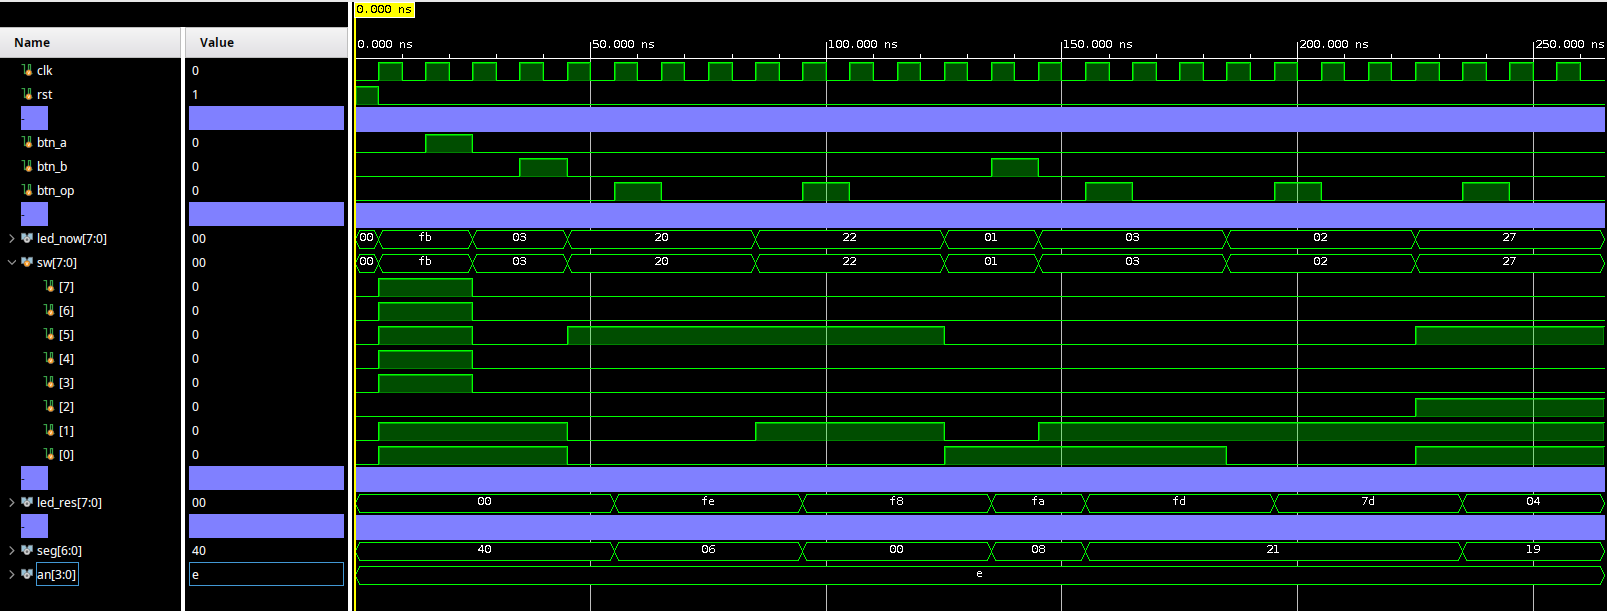
\includegraphics[width=\textwidth]{img/simulacion.png}
    \caption{Forma de onda de la simulación del \textit{testbench}.}
    \label{fig:simulacion_tb}
\end{figure}